\documentclass[10pt,mathserif]{beamer}

\usepackage{graphicx,amsmath,amssymb,psfrag,mathtools}
\usepackage{soul}
\usepackage{amsmath,amsfonts,amsthm,bbm}
\usepackage{stmaryrd}
\usepackage{subcaption}



%Code block environment
\usepackage{listings}


\definecolor{lightgrey}{gray}{0.8}
\definecolor{medgrey}{gray}{0.6}
\definecolor{darkgrey}{gray}{0.4}
\usepackage{xcolor}
\lstset { %
    backgroundcolor=\color{black!5}, % set backgroundcolor
    basicstyle=\ttfamily,
    showstringspaces=false,
    commentstyle = \ttfamily,
    commentstyle=\color{commentgreen}\ttfamily,
    morecomment=[l][\color{darkgrey}]{//},
}



\usepackage{tikz}
\usetikzlibrary{matrix,chains,positioning,decorations.pathreplacing,arrows}
\usetikzlibrary{positioning,calc}
\usepackage{tkz-euclide}
%\usetkzobj{all}





%-------------------------------------------------------------------------------
%Definition of operator font
 \usepackage[bb=boondox]{mathalfa}
%% import \varmathbb without affecting other fonts
\usepackage{xparse}
\DeclareFontFamily{U}{ntxmia}{}
\DeclareFontShape{U}{ntxmia}{m}{it}{<-> ntxmia }{}
\DeclareFontShape{U}{ntxmia}{b}{it}{<-> ntxbmia }{}
\DeclareSymbolFont{lettersA}{U}{ntxmia}{m}{it}
\SetSymbolFont{lettersA}{bold}{U}{ntxmia}{b}{it}
\ExplSyntaxOn
\NewDocumentCommand{\varmathbb}{m}
 {
  \tl_map_inline:nn { #1 }
   {
    \use:c { varbb##1 }
   }
 }
\tl_map_inline:nn { ABCDEFGHIJKLMNOPQRSTUVWXYZ }
 {
  \exp_args:Nc \DeclareMathSymbol{varbb#1}{\mathord}{lettersA}{\int_eval:n { `#1+67 }}
 }
\exp_args:Nc \DeclareMathSymbol{varbbk}{\mathord}{lettersA}{169}
\ExplSyntaxOff
%%
\makeatletter
\DeclareFontFamily{U}{tipa}{}
\DeclareFontShape{U}{tipa}{m}{n}{<->tipa10}{}
\newcommand{\arc@char}{{\usefont{U}{tipa}{m}{n}\symbol{62}}}%

\newcommand{\arc}[1]{\mathpalette\arc@arc{#1}}

\newcommand{\arc@arc}[2]{%
  \sbox0{$\m@th#1#2$}%
  \vbox{
    \hbox{\resizebox{\wd0}{\height}{\arc@char}}
    \nointerlineskip
    \box0
  }%
}
\makeatother
\newcommand{\opA}{{\varmathbb{A}}}
\newcommand{\opB}{{\varmathbb{B}}}
\newcommand{\opC}{{\varmathbb{C}}}
\newcommand{\opD}{{\varmathbb{D}}}
\newcommand{\opE}{{\varmathbb{E}}}
\newcommand{\opF}{{\varmathbb{F}}}
\newcommand{\opG}{{\varmathbb{G}}}
\newcommand{\opH}{{\varmathbb{H}}}
\newcommand{\opI}{{\varmathbb{I}}}
\newcommand{\opJ}{{\varmathbb{J}}}
\newcommand{\opK}{{\varmathbb{K}}}
\newcommand{\opL}{{\varmathbb{L}}}
\newcommand{\opM}{{\varmathbb{M}}}
\newcommand{\opN}{{\varmathbb{N}}}
\newcommand{\opO}{{\varmathbb{O}}}
\newcommand{\opP}{{\varmathbb{P}}}
\newcommand{\opQ}{{\varmathbb{Q}}}
\newcommand{\opR}{{\varmathbb{R}}}
\newcommand{\opS}{{\varmathbb{S}}}
\newcommand{\opT}{{\varmathbb{T}}}
\newcommand{\opU}{{\varmathbb{U}}}
\newcommand{\opV}{{\varmathbb{V}}}
\newcommand{\opW}{{\varmathbb{W}}}
\newcommand{\opX}{{\varmathbb{X}}}
\newcommand{\opY}{{\varmathbb{Y}}}
\newcommand{\opZ}{{\varmathbb{Z}}}
\newcommand{\opZer}{\mathbb{0}}
%-------------------------------------------------------------------------------



%-------------------------------------------------------------------------------
%Definition of other font types
\newcommand{\va}{{\mathbf{a}}}
\newcommand{\vb}{{\mathbf{b}}}
\newcommand{\vc}{{\mathbf{c}}}
\newcommand{\vd}{{\mathbf{d}}}
\newcommand{\ve}{{\mathbf{e}}}
\newcommand{\vf}{{\mathbf{f}}}
\newcommand{\vg}{{\mathbf{g}}}
\newcommand{\vh}{{\mathbf{h}}}
\newcommand{\vi}{{\mathbf{i}}}
\newcommand{\vj}{{\mathbf{j}}}
\newcommand{\vk}{{\mathbf{k}}}
\newcommand{\vl}{{\mathbf{l}}}
\newcommand{\vm}{{\mathbf{m}}}
\newcommand{\vn}{{\mathbf{n}}}
\newcommand{\vo}{{\mathbf{o}}}
\newcommand{\vp}{{\mathbf{p}}}
\newcommand{\vq}{{\mathbf{q}}}
\newcommand{\vr}{{\mathbf{r}}}
\newcommand{\vs}{{\mathbf{s}}}
\newcommand{\vt}{{\mathbf{t}}}
\newcommand{\vu}{{\mathbf{u}}}
\newcommand{\vv}{{\mathbf{v}}}
\newcommand{\vw}{{\mathbf{w}}}
\newcommand{\vx}{{\mathbf{x}}}
\newcommand{\vy}{{\mathbf{y}}}
\newcommand{\vz}{{\mathbf{z}}}

\newcommand{\vA}{{\mathbf{A}}}
\newcommand{\vB}{{\mathbf{B}}}
\newcommand{\vC}{{\mathbf{C}}}
\newcommand{\vD}{{\mathbf{D}}}
\newcommand{\vE}{{\mathbf{E}}}
\newcommand{\vF}{{\mathbf{F}}}
\newcommand{\vG}{{\mathbf{G}}}
\newcommand{\vH}{{\mathbf{H}}}
\newcommand{\vI}{{\mathbf{I}}}
\newcommand{\vJ}{{\mathbf{J}}}
\newcommand{\vK}{{\mathbf{K}}}
\newcommand{\vL}{{\mathbf{L}}}
\newcommand{\vM}{{\mathbf{M}}}
\newcommand{\vN}{{\mathbf{N}}}
\newcommand{\vO}{{\mathbf{O}}}
\newcommand{\vP}{{\mathbf{P}}}
\newcommand{\vQ}{{\mathbf{Q}}}
\newcommand{\vR}{{\mathbf{R}}}
\newcommand{\vS}{{\mathbf{S}}}
\newcommand{\vT}{{\mathbf{T}}}
\newcommand{\vU}{{\mathbf{U}}}
\newcommand{\vV}{{\mathbf{V}}}
\newcommand{\vW}{{\mathbf{W}}}
\newcommand{\vX}{{\mathbf{X}}}
\newcommand{\vY}{{\mathbf{Y}}}
\newcommand{\vZ}{{\mathbf{Z}}}

\newcommand{\cA}{{\mathcal{A}}}
\newcommand{\cB}{{\mathcal{B}}}
\newcommand{\cC}{{\mathcal{C}}}
\newcommand{\cD}{{\mathcal{D}}}
\newcommand{\cE}{{\mathcal{E}}}
\newcommand{\cF}{{\mathcal{F}}}
\newcommand{\cG}{{\mathcal{G}}}
\newcommand{\cH}{{\mathcal{H}}}
\newcommand{\cI}{{\mathcal{I}}}
\newcommand{\cJ}{{\mathcal{J}}}
\newcommand{\cK}{{\mathcal{K}}}
\newcommand{\cL}{{\mathcal{L}}}
\newcommand{\cM}{{\mathcal{M}}}
\newcommand{\cN}{{\mathcal{N}}}
\newcommand{\cO}{{\mathcal{O}}}
\newcommand{\cP}{{\mathcal{P}}}
\newcommand{\cQ}{{\mathcal{Q}}}
\newcommand{\cR}{{\mathcal{R}}}
\newcommand{\cS}{{\mathcal{S}}}
\newcommand{\cT}{{\mathcal{T}}}
\newcommand{\cU}{{\mathcal{U}}}
\newcommand{\cV}{{\mathcal{V}}}
\newcommand{\cW}{{\mathcal{W}}}
\newcommand{\cX}{{\mathcal{X}}}
\newcommand{\cY}{{\mathcal{Y}}}
\newcommand{\cZ}{{\mathcal{Z}}}
%-------------------------------------------------------------------------------




%-------------------------------------------------------------------------------
%% macros for math notions and operators
\newcommand{\EE}{{\mathbb{E}}}
\newcommand{\expec}{\mathbb{E}}
\newcommand{\Prob}{{\mathrm{Prob}}} % probability

\newcommand{\reals}{\mathbb{R}}
\newcommand{\RR}{\mathbb{R}}
\newcommand{\complex}{\mathbb{C}}
\newcommand{\CC}{\mathbb{C}}
\newcommand{\nats}{\mathbb{N}}
\newcommand{\NN}{\mathbb{N}}
\newcommand{\ZZ}{\mathbb{Z}}
\newcommand{\bigO}{\mathcal{O}}
\newcommand{\order}[1]{{\mathcal{O}\left(#1\right)}}
\renewcommand{\SS}{{\mathbb{S}}}
\newcommand{\SSp}{\mathbb{S}_{+}}
\newcommand{\SSpp}{\mathbb{S}_{++}}
\newcommand{\sign}{\mathrm{sign}}
\newcommand{\vzero}{\mathbf{0}}
\newcommand{\vone}{{\mathbf{1}}}

\renewcommand{\Re}{\operatorname{Re}} 	%Real part
\renewcommand{\Im}{\operatorname{Im}}	%imaginary part

%\newcommand{\supp}{{\mathrm{supp}}} % support
\newcommand{\range}{\mathrm{range}\,} % domain
\newcommand{\tr}{{\mathrm{tr}}} % trace
%-------------------------------------------------------------------------------





%-------------------------------------------------------------------------------
%% Theorem definitions
\setbeamertemplate{theorems}[ams style] 
\newtheorem*{theorem*}{Theorem}
%\newtheorem{lemma}{Lemma}    % already provided by amsthm
\newtheorem{proposition}{Proposition}
%\newtheorem{proof}{Proof}  % already provided by amsthm


%-------------------------------------------------------------------------------
%% operator and convex analysis definitions

\newcommand*{\fix}{\mathrm{Fix}\,}
\newcommand*{\zer}{\mathrm{Zer}\,}
\newcommand*{\gra}{\mathrm{Gra}\,}
\newcommand{\prox}{\mathrm{Prox}}
\newcommand{\proj}{\Pi}
\newcommand{\aff}{\mathrm{aff}\,}    %affine hull
\newcommand{\intr}{\mathrm{int}\,}   %interior
\newcommand{\relint}{\mathrm{ri}\,}  %relative interior
\newcommand{\dom}{\mathrm{dom}\,} % domain
\newcommand{\epi}{\mathrm{epi}\,} % epigraph
\newcommand{\dist}{\mathrm{dist}}
\newcommand{\lagrange}{\mathbf{L}}  %saddle function
\newcommand{\fitzpatrick}{\mathbf{F}}   %Fitzpatrick function
\newcommand{\vecdelay}{\boldsymbol{d}}   %vector delay
\DeclareMathOperator*{\argmin}{argmin}
\DeclareMathOperator*{\argmax}{argmax}

%-------------------------------------------------------------------------------
%SRG definitions
\newcommand{\ereal}{\overline{\mathbb{R}^2}}
\newcommand{\ecomplex}{\overline{\mathbb{C}}}
\newcommand{\binfty}{{\boldsymbol \infty}}
\newcommand{\rarc}{\mathrm{Arc}^+}
\newcommand{\larc}{\mathrm{Arc}^-}


%-------------------------------------------------------------------------------




%-------------------------------------------------------------------------------
%Miscellaneous Stuff
%% sequences
\newcommand{\itom}{_{i=1}^{m}}
\newcommand{\ieqm}{i=1,\dots,m}

% use \numberthis to add an equation number in align*
\newcommand\numberthis{\addtocounter{equation}{1}\tag{\theequation}}

\newcolumntype{P}[1]{>{\centering\arraybackslash}p{#1}}

\mode<presentation>
{
\usetheme{default}
}
\setbeamertemplate{navigation symbols}{}
\usecolortheme[rgb={0.13,0.28,0.59}]{structure}
\setbeamertemplate{itemize subitem}{--}
\setbeamertemplate{frametitle} {
	\begin{center}
	  {\large\bf \insertframetitle}
	\end{center}
}

\newcommand\footlineon{
  \setbeamertemplate{footline} {
    \begin{beamercolorbox}[ht=2.5ex,dp=1.125ex,leftskip=.8cm,rightskip=.6cm]{structure}
      \footnotesize \insertsection
      \hfill
      {\insertframenumber}
    \end{beamercolorbox}
    \vskip 0.45cm
  }
}
\footlineon


\newcommand\footlineoff{
  \setbeamertemplate{footline} {
    \begin{beamercolorbox}[ht=2.5ex,dp=1.125ex,leftskip=.8cm,rightskip=.6cm]{structure}
      \footnotesize 
      \hfill
      {\insertframenumber}
    \end{beamercolorbox}
    \vskip 0.45cm
  }
}


\newcommand\blfootnote[1]{%
  \begingroup
  \renewcommand\thefootnote{}\footnote{#1}%
  \addtocounter{footnote}{-1}%
  \endgroup
}


\AtBeginSection[] 
{ 
	\begin{frame}<beamer> 
		\frametitle{Outline} 
		\tableofcontents[currentsection,currentsubsection] 
	\end{frame} 
} 

%% wotao's preference

        % itemize, black bullet, %150 spacing between items using "witemize"
        \newenvironment{witemize}{\itemize\addtolength{\itemsep}{0.3\baselineskip}}{\enditemize}

\iffalse
        % \setbeamertemplate{itemize items}[square]
        \setbeamertemplate{itemize items}{\textbullet}
        \setbeamercolor{itemize item}{fg=black}
        \setbeamercolor{itemize subitem}{fg=black}
        \setbeamercolor{itemize subsubitem}{fg=black}
        \setbeamercolor{enumerate item}{fg=black}
        \setbeamercolor{enumerate subitem}{fg=black}
        \setbeamercolor{enumerate subsubitem}{fg=black}
        \setbeamertemplate{itemize/enumerate body begin}{\normalsize}
        \setbeamertemplate{itemize/enumerate subbody begin}{\normalsize}
        \setbeamertemplate{itemize/enumerate subsubbody begin}{\normalsize}

        % itemize enumerate use normal sized texts
        \setbeamertemplate{itemize/enumerate body begin}{\normalsize}
        \setbeamertemplate{itemize/enumerate subbody begin}{\normalsize}
        \setbeamertemplate{itemize/enumerate subsubbody begin}{\normalsize}

        % block, black over gray with no shadow
        \setbeamertemplate{blocks}[rounded][shadow=false]
        \setbeamercolor{block title}{fg=black,bg=gray!40}
        \setbeamercolor{block body}{fg=black,bg=gray!10}
\fi

\author{Ernest K. Ryu and Wotao Yin}

\date{Large-Scale Convex Optimization via Monotone Operators}


\title{\large \bfseries Introduction and Preliminaries}


\begin{document}

\frame{
\thispagestyle{empty}
\titlepage
}


\section{Introduction}
\begin{frame}
\frametitle{Convex optimization via monotone operators}
Monotone operator theory is an elegant and powerful tool.

\vspace{0.2in}

We use this tool to provide a unified analysis of \textbf{many} classical and modern first-order convex optimization methods.

\end{frame}

\begin{frame}
\frametitle{Optimization methods to cover}
\begin{itemize}
\item[\S2] Gradient descent,
dual ascent, proximal point method, method of multipliers,
proximal method of multipliers, forward-backward splitting, Douglas--Rachford splitting, Davis--Yin splitting, 
proximal gradient method, iterative soft thresholding, consensus optimization, forward-Douglas--Rachford, variable metric proximal point, variable metric forward-backward splitting,
backward-backward method.
%.
\item[\S3] 
ADMM,
alternating minimization algorithm (Tseng),
PDHG (Chambolle--Pock),
Condat--V\~u,
proximal method of multipliers with function lineraization,
PAPC/PDFP$^2$O,
linearized method of multipliers,
PD3O,
proximal ADMM,
linearized ADMM,
DYS 3-block ADMM,
doubly linearized method of multipliers.
%.
\item[\S5]
Coordinate gradient descent
block-coordinate descent,
coordinate proximal-gradient descent,
stochastic dual coordinate ascent,
MISO/finito,
coordinate updates on conic programs.
\item[\S6] 
ARock,
asynchronous coordinate gradient descent,
asynchronous ADMM.
\end{itemize}
\end{frame}



\begin{frame}
\frametitle{Optimization methods to cover}
\begin{itemize}
\item[\S7]
Stochastic forward-backward method,
stochastic gradient descent,
stochastic proximal gradient method,
stochastic proximal simultaneous gradient method,
stochastic Condat--V\~u.
\item[\S8]
Function-linearized proximal ADMM,
golden ratio ADMM, 
doubly-linearized ADMM,
partial linearization,
near-circulant splitting,
Jacobi ADMM,
2-1-2 ADMM,
Trip-ADMM,
split Bregman method,
four-block 2-1-2-4-3-4 ADMM.
\item[\S11] 
Distributed ADMM, decentralized ADMM, distributed gradient descent, method of diffusion, adapt-then-combine, PG-EXTRA, NIDS.
\item[\S12]
Nesterov accelerated gradient method, 
FISTA,
accelerated proximal point method.
\end{itemize}
\end{frame}




\begin{frame}
\frametitle{1st-order vs.\ 2nd-order methods}
2nd-order methods:
\begin{itemize}
\item 
Use second-order derivatives or their approximations.
\item
Focus of 70s--90s. Effective for smaller problems.
\item
Require fewer iterations to solve the optimization problem to high accuracy, even up to machine precision.
\end{itemize}

1st-order methods:
\begin{itemize}
\item 
Can be described and analyzed with gradients and subgradients.
\item
Current focus. Effective for larger problems.
\item
Lower computational cost per iteration.
For large problems, one iteration of a 2nd-order method is infeasible, while 1st-order methods can solve to acceptable accuracy.
\item
1st-order methods are extremely simple; 2- or 3-line description.
Simpler methods are easy to try out and to parallelize.
\end{itemize}

\end{frame}







\begin{frame}
\frametitle{1st-order vs.\ 2nd-order methods}
Two class of methods are usually not in competition.


\begin{itemize}
\item
When a high-accuracy solution is needed, second-order methods should be used.
For small problems, use second-order methods, since no reason to forgo the high accuracy.
\item 
In large-scale problems, one should use first-order methods and tolerate inaccuracy.
Most engineering applications only require a few digits of accuracy in its solution.
\end{itemize}


\end{frame}

\begin{frame}
\frametitle{Convergence and convergence rates}
The total cost of a method is
\[
(\text{cost per iteration})\times(\text{number of iterations}).
\]
(cost per iteration): examining the computational cost of the individual components of the method.\\
(number of iterations): analyzing the rate of convergence.


\vspace{0.2in}

In optimization, methods are often compared with cost per iteration.
(We just made this very argument.)
However, a method with a low cost per iteration has the potential, not a guarantee, to be efficient.


\vspace{0.2in}

Nevertheless, focusing on the cost per iteration is a useful simplification.
We focus on establishing convergence without paying much attention to the rate of convergence.
\end{frame}





\begin{frame}
\frametitle{Limitations of monotone operator theory}
We provide streamlined convergence proofs and only discuss results that fit this approach.
Such results are simple but often not the strongest.
%The strongest results in convex optimization usually involve arguments that go beyond monotone operator theory.

\vspace{0.2in}

Proofs based on monotone operator theory use monotonicity, rather than convexity, as the key property.
This line of analysis does not lead to results involving function values.
For example, the gradient method $x^{k+1}=x^k-\alpha\nabla f(x^k)$ converges, under suitable assumptions, with rate $\|\nabla f(x^k)\|^2\le \mathcal{O}(1/k)$ 
(proved with monotonicity)
and $f(x^k)-f(x^\star)\le \mathcal{O}(1/k)$
(proved with convexity).

\vspace{0.2in}
Convex optimization theory goes beyond monotone operators, although monotone operators do play a central role.

\end{frame}


\section{Preliminaries}
\begin{frame}
\frametitle{Overloaded set notation}
We overload many standard notation defined for points to sets:\\
For $\alpha\in \reals$, $x\in \reals^n$,  $A,B\subseteq \reals^n$, $M\in \reals^{m\times n}$:
\begin{align*}
\alpha A&=\{\alpha a\,|\,a\in A\}\\
x+A&=\{x+a\,|\,a\in A\}\\
MA&=\{Ma\,|\,a\in A\}\\
A+B&=\{a+b\,|\,a\in A,\,b\in B\}
\end{align*}
%These operations preserve convexity; if $A$ and $B$ are convex, all of these sets are convex.
\vspace{0.2in}

The sum $A+B$ is called the Minkowski sum.

\end{frame}



\begin{frame}
\frametitle{Schur complement}
Consider
\[
X=
\begin{bmatrix}
A&B\\
B^\intercal&C
\end{bmatrix}\in \reals^{(m+n)\times (m+n)},
\]
where $A=A^\intercal\in \reals^{m\times m}$, $B\in \reals^{m\times n}$, and
$C=C^\intercal\in \reals^{n\times n}$.
When $A$ is invertible,
\[
C-B^\intercal A^{-1}B\in \reals^{n\times n}
\]
is the Schur complement of $A$ in $X$.

\vspace{0.2in}

If $A\succ 0$, then [$X\succ 0$] $\Leftrightarrow$ [$C-B^\intercal A^{-1}B\succ 0$].\\
If $A\succ 0$, then [$X\succeq 0$] $\Leftrightarrow$ [$C-B^\intercal A^{-1}B\succeq 0$].


\vspace{0.2in}

With Schur complement of $C$ in $X$:\\
If $C\succ 0$, then [$X\succ 0$] $\Leftrightarrow$ [$A-BC^{-1}B^\intercal \succ 0$].\\
If $C\succ 0$, then [$X\succeq 0$] $\Leftrightarrow$ [$A-BC^{-1}B^\intercal\succeq 0$].

\vspace{0.2in}
Use Schur complement to assess positive (semi)definiteness.
\end{frame}


\begin{frame}
\frametitle{Lipschitz continuity}
 $\opT\colon \reals^n\rightarrow\reals^m$ is $L$-Lipschitz (continuous) if
\[
\|\opT (x)-\opT (y)\|\le L\|x-y\|\qquad\forall\,x,y\in \reals^n.
\]
%\vspace{0.2in}
$\opT $ is Lipschitz (continuous) if $L$-Lipschitz for some $L\in (0,\infty)$.
%(An operator is $0$-Lipschitz if it is a constant.)


\vspace{0.2in}

\begin{itemize}
\item
If $\opT$ is Lipschitz,  it is continuous.
\item
If $\opT _1$ and $\opT _2$ are $L_1$- and $L_2$-Lipschitz, then
$\opT _1\circ \opT _2$ is $L_1L_2$-Lipschitz.
%\[
%\|\opT _1(\opT _2(x))-\opT _1(\opT _2(y))\|
%\le
%L_1\|\opT _2(x)-\opT _2(y)\|
%\le
%L_1L_2\|x-y\|.
%\]
\item
If $\opT _1$ and $\opT _2$ are  $L_1$- and $L_2$-Lipschitz, then
$\alpha_1\opT _1+\alpha_2 \opT _2$ is $(|\alpha_1|L_1+|\alpha_2|L_2)$-Lipschitz.
\end{itemize}
\end{frame}


\begin{frame}
\frametitle{Interior}
Closed ball of radius $r$ centered at $x$:
\[
B(x,r)=\{y\in \reals^n\,|\,\|y-x\|\le r\}
\]

\vspace{0.2in}

Interior of $C\subseteq\reals^n$:
\[
\intr C = \{x\in C\,|\,
B(x,r)\subseteq C\text{ for some } r>0
\}
\]


\vspace{0.1in}

Closure of $C\subseteq\reals^n$: $\mathrm{cl}\, C$

\vspace{0.2in}
Boundary of $C\subseteq\reals^n$:  $\mathrm{cl}\, C\backslash \intr C$
\end{frame}

\begin{frame}
\frametitle{Relative interior}
Affine set:
$x_0+V$, where $x_0\in \reals^n$ and $V\subseteq\reals^n$ is a subspace.

\vspace{0.2in}

Affine hull of $C\subseteq\reals^n$:
\[
\aff C=\{\theta_1x_1+\dots+\theta_kx_k\,|\,x_1,\dots,x_k\in C,\,\theta_1+\dots+\theta_k=1,\,k\ge 1\}
\]
Affine hull is the smallest affine set containing $C$.

\vspace{0.2in}

Relative interior of $C\subset\reals^n$:
\[
\relint C = \{x\in C\,|\,B(x,r)\cap \aff C\subseteq C\text{ for some } r>0\}
\]
$\relint C$ of a nonempty convex set $C$ is nonempty.

\vspace{0.2in}

Relative boundary of $ C\subseteq\reals^n$: $\mathrm{cl}\, C\backslash \relint C$
\vspace{0.2in}


%When  dealing with low-dimensional sets placed in higher-dimensional spaces, the notion of relative interior is useful.

\end{frame}

\begin{frame}
\frametitle{Relative interior example}
%Consider the line segment
\[
S=\left\{(x,y)\in \reals^2\,|\,x\in[0.5,1],\,y=4x-3\right\}.
\]
\vspace{0.1in}
\begin{center}
\begin{tabular}{cc}
\raisebox{-.5\height}{
\begin{tikzpicture}[scale=1.2]
\draw[line width=1.0pt] (0.5,-1)--(1,1);
\draw (0.9,0.65) node[left] {$S=$};
\draw [<->] (-1,0) -- (1.5,0);
\draw [<->] (-0,-1.2) -- (-0,1.2);
\end{tikzpicture}}
&
\raisebox{-.5\height}{
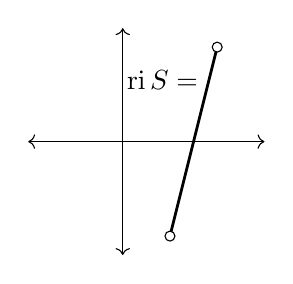
\begin{tikzpicture}[scale=1.2]
\draw[line width=1.0pt] (0.5,-1)--(1,1);
\filldraw [fill=white](0.5,-1) circle ({1.5pt});
\filldraw [fill=white](1,1)circle ({1.5pt});
\draw (0.9,0.65) node[left] {$\relint S=$};
\draw [<->] (-1,0) -- (1.5,0);
\draw [<->] (-0,-1.2) -- (-0,1.2);
\end{tikzpicture}}
\end{tabular}
\end{center}
\end{frame}


\begin{frame}
\frametitle{Functions}
Extended-valued functions map $\reals^n$ to the extended real line $ \RR\cup\{\pm\infty\}$.
(Some saddle functions have value $\pm\infty$.)

\vspace{0.2in}

(Effective) domain of $f$:
\[
\dom f = \{x\in \reals^n\,|\,f(x)<\infty\}
\]


\vspace{0.2in}

$f$ is convex if $\dom f $ is convex and
\[
    f(\theta x  + (1-\theta)y ) \le \theta f(x ) + (1-\theta)f(y ),\quad\forall\, x ,y \in\dom f,~\theta\in(0,1).
\]
$f$ is strictly convex if the inequality is strict when $x \ne y $.
$f$ is (strictly) concave if $-f$ is (strictly) convex.

\vspace{0.2in}

To clarify, we say $f\colon\reals^n\rightarrow \RR\cup\{\pm\infty\}$ is differentiable if
$f\colon\reals^n\rightarrow \RR$ (so $f$ is not extended-valued) and $\frac{\partial f}{\partial x_i}(x)$ exists for all $x\in \reals^n$, $i=1,\dots,n$.


\end{frame}

\begin{frame}
\frametitle{CCP functions}
$f$ is CCP if closed, convex, and proper:
\begin{itemize}
\item
$f$ is proper if $f(x)=-\infty$ never and $f(x)<\infty$ somewhere.
\item
Proper $f$ is closed if epigraph of $f$
\[
    \epi f = \{(x ,\alpha)\in\RR^n\times \RR\,|\, f(x )\le \alpha\}
\]
 is closed.
\end{itemize}
\vspace{0.2in}

Properties:
\begin{itemize}
\item
Most convex functions of interest are closed and proper.
\item

[$f$ is convex] $\Leftrightarrow$ [$\epi f$ is convex]
\item
For proper $f$,  [$f$ closed] $\Leftrightarrow$ [$f$ is lower semi-continuous]
\item

[$f$ CCP]  $\Leftrightarrow$  [$\epi f$ nonempty closed convex without a vertical line]
\end{itemize}
vertical line = $\{x_0\}\times\reals$.


\end{frame}

%\begin{frame}
%\frametitle{CCP functions}
%XXX
%Extended value extension
%XXX
%
%Epigraph of $f$:
%\[
%    \epi f = \{(x ,\alpha)\in\RR^n\times \RR: f(x )\le \alpha\}.
%\]
%$f$ is convex $\Leftrightarrow$ $\epi f$ is convex.
%
%\vspace{0.2in}
%$f$ is proper if $f(x)=-\infty$ never and $f(x)<\infty$ somewhere.
%
%\vspace{0.2in}
%
%Proper $f$ is closed if $\epi f$ is closed. \\
%For proper $f$,  [$f$ closed] $\Leftrightarrow$ [$f$ is lower semi-continuous].
%
%
%\vspace{0.2in}
%
%$f$ is CCP if it is closed, convex, and proper.
%Most convex functions of interest are closed and proper.
%
%\vspace{0.2in}
%
%$f$ CCP  $\Leftrightarrow$  $\epi f$ nonempty closed convex.
%\end{frame}





\begin{frame}
\frametitle{CCP function example}
%Whether a convex function $f$ is closed is determined by $f$'s behavior on the boundary of $\dom f$.
%\vspace{0.1in}
\begin{center}
\begin{tabular}{ccc}
\raisebox{-.5\height}{
\begin{tikzpicture}[scale=1.2]
\draw plot[smooth, tension=.7] coordinates {(0.2,0.5) (1,0.3) (1.8,1.0)};
%\draw[dashed] (0.2,0.5) -- (0.2,2.0);
%\draw[dashed] (1.8,1.0) -- (1.8,2.0);
\draw [<->] (-0.5,0) -- (2,0);
\draw [<->] (0,-0.5) -- (0,2);
\filldraw (0.2,0.5) circle ({1pt});
\filldraw (1.8,1.0) circle ({1pt});
\draw (0,-0.5) node { \phantom{A} };
\end{tikzpicture}}
&\qquad\qquad&
\raisebox{-.5\height}{
\begin{tikzpicture}[scale=1.2]
\draw plot[smooth, tension=.7] coordinates {(0.2,0.5) (1,0.3) (1.8,1.0)};
\draw[dashed] (0.2,0.5) -- (0.2,2.0);
%\draw[dashed] (1.8,1.0) -- (1.8,2.0);
\draw [<->] (-0.5,0) -- (2,0);
\draw [<->] (0,-0.5) -- (0,2);
\filldraw [fill=white](0.2,0.5) circle ({1pt});
\filldraw (1.8,1.0) circle ({1pt});
\draw (0,-0.5) node { \phantom{A} };
\end{tikzpicture}}\\
Closed convex function && Convex but not closed
\end{tabular}
\end{center}

\vspace{0.1in}

The dashed line denotes the function value of $\infty$.
\end{frame}


\begin{frame}
\frametitle{CCP function example}
Epigraph of the CCP $-\log$ is a nonempty closed convex set.
\vspace{0.1in}
\begin{center}
\raisebox{-.5\height}{
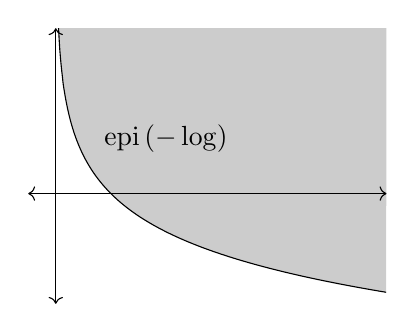
\begin{tikzpicture}[scale=.7]
\begin{scope}
\clip (0,3) rectangle (6,-2);
\fill[fill=lightgrey, domain=0.001:6, variable=\x,samples=500] (0,6) -- plot ({\x},{-ln(\x)}) -- (6,3);
\draw[domain=0.001:6, variable=\x,samples=500] plot ({\x},{-ln(\x)});
\end{scope}
\draw (2,1) node {$\epi (-\log)$};
\draw [<->] (-0.5,0) -- (6,0);
\draw [<->] (0,-2) -- (0,3);
\end{tikzpicture}}
\end{center}
\end{frame}

\begin{frame}
\frametitle{Operations preserving CCP}
If $f$ and $g$ are CCP functions, $\alpha>0$, and $A$ is a matrix, then
\begin{itemize}
\item
$\alpha f$ is CCP
\item
$f+g$ is CCP provided that $\exists\,x$ such that $f(x)+g(x)<\infty$
\item
$f(Ax)$ is CCP provided that $\exists\,x$ such that $f(Ax)<\infty$
\end{itemize}
\end{frame}

\begin{frame}
\frametitle{Indicator function}
For $S\subseteq\RR^n$,
define the \emph{indicator function}
\[
    \delta_S(x) = \begin{cases}
        0& \text{if}~x\in S\\
        \infty& \text{otherwise.}
    \end{cases}
\]
If $S$ is convex, closed, and nonempty, then $\delta_S$ is CCP.
\end{frame}

\begin{frame}
\frametitle{Argmin}
Set of minimizers of $f$:
\[
\argmin f=\left\{x\in \reals^n\,\bigg|\, f(x)=\inf_{z\in \reals^n}f(z)\right\}
\]
%The set $\argmin f$ can be empty, have a single point, or have many points.
\vspace{0.2in}

When $f$ is CCP, $\argmin f$ is closed convex, possibly empty.
\vspace{0.2in}


When $f$ is strictly convex, $\argmin f$ has at most one point.
\end{frame}


\begin{frame}
\frametitle{Subgradient}
$g\in \reals^n$ is a \emph{subgradient} of convex $f$ at $x$ if
\[
f(y) \geq f(x) + \langle g,y-x\rangle\qquad\forall\,y\in \reals^n.
\]
%In other words, a subgradient provides an global affine lower bound of $f$.
%We call \eqref{eq:subgrad-ineq} the \emph{subgradient inequality}.
%\index{subgradient inequality}
%\vspace{0.1in}

The \emph{subdifferential} of convex $f$ at $x$ is
\[
\partial f(x) = \{g\in \reals^n\,|\,f(y) \geq f(x) + \langle g,y-x\rangle,
\,\forall\,y\in \reals^n
\},
\]
i.e., $\partial f(x)=\{\text{subgradients of $f$ at $x$}\}$.

\vspace{0.2in}
\begin{itemize}
\item
$\partial f(x)$ is closed convex
%When $f$ is convex, $\partial f(x)\neq \emptyset$ for any $x \in \relint \dom f$.
\item

[Convex $f$ is differentiable at $x$]
 $\Leftrightarrow$ [$\partial f(x)$ is a singleton]
%If f is L-Lipschitz, then the norm of any of its subgradients is no more than L.
%This should go in the subgradient methods section
\item

[$x^\star\in \argmin f$] $\Leftrightarrow$ [$0\in \partial f(x^\star)$]
\end{itemize}

%(For convex functions, local affine lower bound is a global lower bound.)
\end{frame}


\begin{frame}
\frametitle{Subdifferential example}
The absolute value function is differentiable everywhere except at $0$.

\begin{center}
\begin{tabular}{ccc}
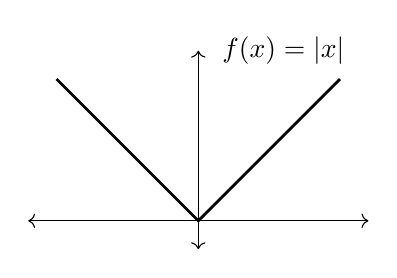
\begin{tikzpicture}[scale=1.8]
\draw[line width = 1pt] (-1,1)--(0,0)--(1,1);
\draw [<->] (-1.2,0) -- (1.2,0);
\draw [<->] (0,-0.2) -- (0,1.2);
\draw (0.6,1.2) node {$f(x)=|x|$};
\end{tikzpicture}
&
\qquad\qquad
&
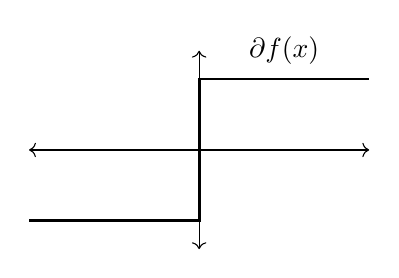
\begin{tikzpicture}[scale=1.8]
\draw[line width = 1pt] (-1.2,-0.5)--(0,-0.5)--(0,0.5)--(1.2,0.5);
\draw [<->] (-1.2,0) -- (1.2,0);
\draw [<->] (0,-0.7) -- (0,0.7);
\draw (0.6,0.7) node {$\partial f(x)$};
\end{tikzpicture}
\end{tabular}
\end{center}
\end{frame}

\begin{frame}
\frametitle{Subdifferential example}
At $x_1$, $f$ is differentiable and $\partial f(x_1)=\{\nabla f(x_1)\}$.\\
At $x_2$, $f$ is not differentiable and has many subgradients.
\begin{center}
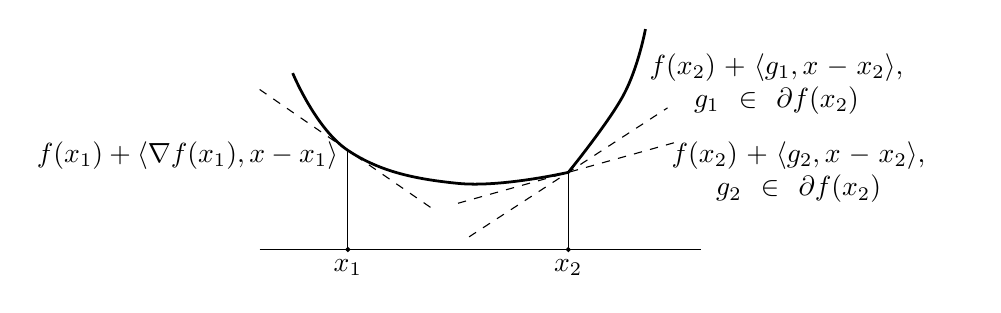
\begin{tikzpicture}[scale=1.4]
%\clip (-1,-0.5) rectangle (2,2);
\draw[line width = 1pt] plot[smooth, tension=.7] coordinates { (-1.2,1.2) (-0.7,0.5) (0.3,0.2) (1.3,0.3)}--plot[smooth, tension=.7] coordinates {(1.3,0.3) (1.8,1) (2,1.6)};
\draw [] (-0.7,0.5) -- (-0.7,-0.4);
\draw [] (1.3,0.3) -- (1.3,-0.4);
%\filldraw (-0.7,0.5) circle ({0.6*1.5/1.2pt});
%\filldraw (1.3,0.3) circle ({0.6*1.5/1.2pt});
\filldraw (-0.7,-0.4) circle ({0.6*1.5/1.8pt});
\filldraw (1.3,-0.4) circle ({0.6*1.5/1.8pt});
\draw (-0.7,-0.4) node[below] {$x_1$};
\draw (1.3,-0.4) node[below] {$x_2$};

\draw (-0.7,0.45) node[left] {$f(x_1)+\langle \nabla f(x_1),x-x_1\rangle$};
\draw (1.6,1.1) node[right,text width=4.2cm, align=center] {$f(x_2)+\langle g_1,x-x_2\rangle$, $g_1\in \partial f(x_2)$};
\draw (1.8,0.3) node[right,text width=4.2cm, align=center] {$f(x_2)+\langle g_2,x-x_2\rangle$, $g_2\in \partial f(x_2)$};

\def\s{-0.69};
\def\x{0.8};
\draw[dashed] ({-0.7-\x},{0.5-\x*\s})--({-0.7+\x},{0.5+\x*\s});
\def\s{0.65};
\def\x{0.9};
\draw[dashed] ({1.3-\x},{0.3-\x*\s})--({1.3+\x},{0.3+\x*\s});
\def\s{0.28};
\def\x{1};
\draw[dashed] ({1.3-\x},{0.3-\x*\s})--({1.3+\x},{0.3+\x*\s});
\draw [] (-1.5,-0.4) -- (2.5,-0.4);
\end{tikzpicture}
\end{center}
\end{frame}




\begin{frame}[plain]
\frametitle{Normal cone operator}
$C \subseteq \reals^n$ closed convex.
Then
\[
\partial \delta_C(x)=\opN_C(x) = \left\{ \begin{array}{ll}
\emptyset & x \not\in C\\
\{ y \;|\; \langle y,z-x\rangle\leq 0~\forall \,z\in C \} &  x \in C
\end{array}\right.
\]
is the normal cone operator.
%For $x\in \intr C$, $\opN_C(x) = \{0\}$, and for $x\notin C$, $\opN_C(x)=\emptyset$; $\opN_C(x)$ is nontrivial only when $x$ is on the boundary of $C$.
\vspace{-0.15in}
\begin{center}
	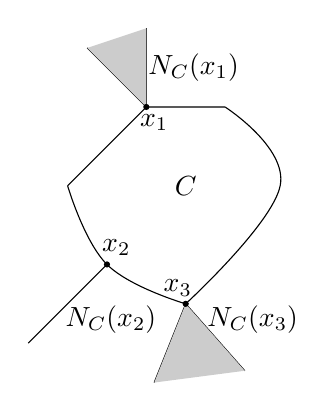
\begin{tikzpicture}[scale=1]
		\draw (-4.5,-0.5) -- (-3.5,0.5) -- (-2.5,0.5);
		\draw plot[smooth, tension=.7] coordinates {(-2.5,0.5) (-1.8,-0.5) (-3,-2)};
		\draw plot[smooth, tension=.7] coordinates {(-3,-2)  (-4.,-1.5) (-4.5,-0.5) };
		\node  at (-3,-0.5) {{$C$}};
		
		\draw  (-4,-1.5) -- (-5,-2.5) ;
		\filldraw (-4,-1.5) circle[radius={0.6*1.5/1pt}];
		\node  at (-3.8812,-1.2893) {{$x_2$}};
		\node  at (-3.95,-2.2) {{$\opN_C(x_2)$}};
		
		\draw  (-3,-2)-- (-3.4,-3.) ;
		\draw  (-3,-2)-- (-2.25,-2.85) ;
		\fill[fill=lightgrey]  (-3,-2)-- (-3.4,-3.)-- (-2.25,-2.85)  ;
		\filldraw (-3,-2) circle[radius={0.6*1.5/1pt}];
		\node  at (-3.1,-1.8) {{$x_3$}};
		\node  at (-2.15,-2.2) {{$\opN_C(x_3)$}};
		
		\draw  (-3.5,0.5)-- (-4.25,1.25) ;
		\draw  (-3.5,0.5)-- (-3.5,1.5) ;
		\fill[fill=lightgrey]  (-3.5,0.5)-- (-4.25,1.25)--(-3.5,1.5);
		\filldraw (-3.5,0.5) circle[radius={0.6*1.5/1pt}];
		\node  at (-3.4,0.3) {{$x_1$}};
		\node  at (-2.9,1) {{$\opN_C(x_1)$}};
	\end{tikzpicture}
	\end{center}
	\vspace{-0.0in}
%The normal cone operator is an important object in convex analysis.
%which is why we point out this connection.
%In this book, we will not pay too much attention to the meaning of $\opN_C$.
We primarily use $\opN_C$ as notational shorthand for $\partial \delta_C$.
\end{frame}

\begin{frame}
\frametitle{Subdifferentiability}
Convex $f$ is subdifferentiable at $x$ if $\partial f(x)\ne \emptyset$.

\vspace{0.2in}
When $f$ is CCP,
\begin{itemize}
\item
$\partial f(x)=\emptyset$ where $x\notin\dom f$
\item
$\partial f(x)\neq \emptyset$ for any $x \in \relint \dom f$
\item
$ f$ may or may not be subdifferentiable on $\dom f\backslash\relint \dom f$
\end{itemize}
\end{frame}


\begin{frame}
\frametitle{Non-subdifferentiable example}
\[
f(x)=
\left\{
\begin{array}{ll}
-\sqrt{x}&\text{ for }x \ge 0\\
\infty&\text{ for }x <0
\end{array}
\right.
\]
is not subdifferentiable at $x=0$,
although $0\in \dom f$ and $f$ is CCP.

% The slope is $-\infty$, but we do not allow infinite gradients.
\vspace{0.1in}
\begin{center}
\raisebox{-.5\height}{
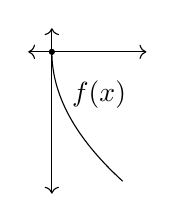
\begin{tikzpicture}[scale=3]
\draw[domain=0:0.3, variable=\x,samples=500] plot ({\x},{-sqrt(\x)});
\draw (0.2,-.18) node {$f(x)$};
\filldraw (0,0) circle ({0.6*1.5/3pt});
\draw [<->] (-0.1,0) -- (0.4,0);
\draw [<->] (0,-0.6) -- (0,0.1);
\end{tikzpicture}}
\end{center}
\end{frame}

\begin{frame}
\frametitle{Subgradient identities}

Several standard identities for gradients also hold for subdifferentials when regularity conditions hold:
\begin{itemize}
\item
$\partial \alpha f=\alpha \partial f$, if $\alpha>0$
\item
$g(x)=f(Ax)$, 
$\partial g=A^\intercal\partial f A$, if $\cR(A)\cap \relint \dom f\ne\emptyset$
\item
$\partial (f+g)=\partial f+\partial g$, if $\dom f\cap \intr\dom g\ne\emptyset$
\end{itemize}
%(Second and third identity not easy to prove.)

\vspace{0.2in}


Without regularity conditions,
\[
\partial g(x)\supseteq A^\intercal\partial f(Ax),
\qquad
\partial (f+g)(x)\supseteq\partial f(x)+\partial g(x)
\]
%(Straightforward to prove.)

\end{frame}

\begin{frame}
\frametitle{Regularity conditions}

Say we have 
``P $\Rightarrow$ Q''.
\vspace{0.2in}

Then, if P ``usually'' holds then Q ``usually'' holds, and we say P is a regularity condition, since P is satisfied in the usual ``regular'' case.

\vspace{0.2in}

Examples:
\begin{itemize}
\item 

[$\dom f\cap \intr\dom g\ne \emptyset$] $\Rightarrow$ [$\partial (f+g)=\partial f+\partial g$].
\item

[Slater's constraint qualification] $\Rightarrow$ [strong duality].
\end{itemize}


\end{frame}




\begin{frame}
\frametitle{Conjugate function}
Conjugate function of $f$:
\[
f^*(y)=\sup_{x\in\reals^n}\left\{\langle y,x\rangle-f(x)\right\}
\]

\vspace{0.2in}

Properties: when $f$ is CCP
\begin{itemize}
\item
$f^*$ is CCP and  $f^{**}=f$
\item
$(\nabla f)^{-1}=\nabla f^*$ when $f$ and $f^*$ are differentiable
\item
$(\partial f)^{-1}=\partial f^*$ in general (more on this next section)
\end{itemize}
\end{frame}

\begin{frame}
\frametitle{Strong convexity}
CCP $f$ is $\mu$-strongly convex if:
\begin{itemize}
\item $f(x)-(\mu/2)\|x\|^2$ is convex.
\item $\langle \partial f(x)-\partial f(y),x-y\rangle \ge \mu\|x-y\|^2$ for all $x,y$.
\item
$\nabla^2f(x)\succeq \mu I$ for all $x$ if $f$ is twice continuously differentiable.
\end{itemize}
These conditions are equivalent.

\vspace{0.2in}

If $f$ is $\mu$-strongly convex and $g$ is convex, then $f+g$ is $\mu$-strongly convex.
%The curvature of a convex function at a nondiffererntiable point is infinite, which is greater than $\mu\in(0,\infty)$.
To clarify, strong convexity does not imply differentiability.
\end{frame}


\begin{frame}
\frametitle{$L$-smooth function}
CCP $f$ is $L$-smooth if:
\begin{itemize}
\item $f(x)-(L/2)\|x\|^2$ is concave.
\item $f$ is differentiable and $\langle \nabla f(x)-\nabla f(y),x-y\rangle
\ge (1/L)
 \|\nabla f(x)-\nabla f(y)\|^2
$ for all $x,y$.
\item $f$ is differentiable and $\nabla f$ is $L$-Lipschitz.
\item
$\nabla^2f(x)\preceq LI$ for all $x$ if $f$ is twice continuously differentiable.
\end{itemize}
These conditions are equivalent.

\vspace{0.2in}

``$L$-smoothness'', which implies once-continuous differentiability,  is somewhat non-standard; ``smoothness'' often means infinite differentiability in other fields of mathematics.
\end{frame}




\begin{frame}
\frametitle{Strong convexity and smoothness}
Informally speaking, $\mu$-strongly convex functions have upward curvature of at least $\mu$ and $L$-smooth convex functions have upward curvature of no more than $L$.
We can think of nondifferentiable points to be points with infinite curvature.


\begin{center}
\begin{tabular}{cc}
\raisebox{-.5\height}{
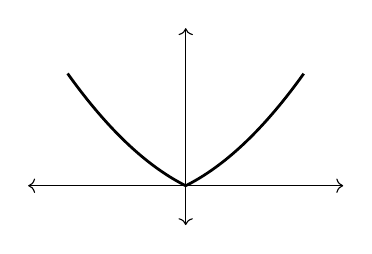
\begin{tikzpicture}[scale=1]
\draw [<->] (-2,0) -- (2,0);
\draw [<->] (-0,-.5) -- (-0,2);
\draw [line width=1pt] plot[domain=-1.5:0, variable=\x,samples=100] ({\x},{-0.5*\x+0.3*(\x)^2}) -- plot[domain=0:1.5, variable=\x,samples=100] ({\x},{0.5*\x+0.3*(\x)^2});
\end{tikzpicture}}
&
\raisebox{-.5\height}{
\begin{tikzpicture}[scale=1]
\draw [<->] (-2,0) -- (2,0);
\draw [<->] (-0,-.5) -- (-0,2);
\draw [line width=1pt] plot[domain=-1.5:-0.5, variable=\x,samples=100] ({\x},{(\x+0.5)^2}) -- plot[domain=0.5:1.5, variable=\x,samples=100] ({\x},{(\x-0.5)^2});
\end{tikzpicture}}
\\
Strongly convex but not smooth & Smooth but not strongly convex.
\end{tabular}
\end{center}
\end{frame}

\begin{frame}
\frametitle{Strong convexity and smoothness}
If $f$ is $\mu$-strongly convex and $L$-smooth, then $\mu\le L$ since
\begin{align*}
\mu\|x-y\|^2&\le \langle \nabla f(x)-\nabla f(y),x-y\rangle\\
&\le \| \nabla f(x)-\nabla f(y)\|\|x-y\|\\
&\le L\|x-y\|^2.
\end{align*}

\vspace{0.2in}
Strong convexity and smoothness are dual properties:\\
if $f$ CCP, [$f$ is $\mu$-strongly convex] $\Leftrightarrow$ [$f^*$ is $(1/\mu)$-smooth]

\end{frame}






\begin{frame}
\frametitle{Convex-concave saddle function and saddle point}
Let $\lagrange\colon\reals^{n}\times\reals^m\rightarrow\reals\cup\{\pm\infty\}$.
We say $\lagrange(x,u)$ is convex-concave if $\lagrange$ is convex in $x$ when $u$ is fixed and concave in $u$ when $x$ is fixed.

\vspace{0.2in}
$(x^\star,u^\star)$ is a saddle point of $\lagrange$ if
\[
\lagrange(x^\star,u)\le \lagrange(x^\star,u^\star)\le \lagrange(x,u^\star)
\qquad\forall\,x\in \reals^n,\,u\in \reals^m.
\]

\end{frame}

\begin{frame}
\frametitle{Duality from saddle functions}
Primal problem generated by $\lagrange$:
\[
\begin{array}{ll}
\underset{x\in \reals^n}{\mbox{minimize}}&\sup_{u\in \reals^m} \lagrange(x,u)
\end{array}
\]
\vspace{0.2in}

%and write $p^\star=\inf_x \sup_u \lagrange(x,u)$ for the primal optimal value.
Dual problem generated by $\lagrange$:
\[
\begin{array}{ll}
\underset{u\in \reals^m}{\mbox{maximize}}&\inf_{x\in \reals^n} \lagrange(x,u)
\end{array}
\]
\vspace{0.2in}

%and write $d^\star=\sup_u\inf_x \lagrange(x,u)$ for the dual optimal value.
%In most engineering settings, one starts with an optimization problem, not a convex-concave saddle function.


Trick is to find $\lagrange$ that generates the primal problem of interest.
\end{frame}


\begin{frame}
\frametitle{Duality example: linearly constrained minimization}
%Let $f$ be a CCP function on $\reals^n$, $A\in \reals^{m\times n}$ and $b\in \reals^m$.
\[
\lagrange(x,u)=f(x)+\langle u, Ax-b\rangle
\]
generates the primal problem
\[
\begin{array}{ll}
\underset{x\in \reals^n}{\mbox{minimize}}&f(x)\\
\mbox{subject to}&Ax=b
\end{array}
\]
and dual problem
\[
\begin{array}{ll}
\underset{u \in \reals^m}{\mbox{maximize}}&-f^*(-A^\intercal u)-b^\intercal u.
\end{array}
\]

\vspace{0.2in}

If 
$\{x\,|\,Ax=b\}\cap \intr \dom f\ne \emptyset$
 holds, then $d^\star=p^\star$.
\end{frame}


\begin{frame}
\frametitle{Duality example: Fenchel--Rockafellar dual}
\[
\lagrange(x,u)=f(x)+\langle u, Ax\rangle-g^*(u)
\]
generates the primal problem
\[
\begin{array}{ll}
\underset{x\in \reals^n}{\mbox{minimize}}&f(x)+g(Ax)
\end{array}
\]
and dual problem
\[
\begin{array}{ll}
\underset{u \in \reals^m}{\mbox{maximize}}&-f^*(-A^\intercal u)-g^*(u).
\end{array}
\]
\vspace{0.2in}

If  
$A\dom f\cap \intr \dom g \ne \emptyset$
 holds, then $d^\star=p^\star$.
\end{frame}



\begin{frame}
\frametitle{Weak and strong duality}
Weak duality: $d^\star\le p^\star$. Always holds.


\vspace{0.2in}
\textbf{Proof.}
For any $x,u$ we have
\begin{gather*}
\inf_x  \lagrange(x,u)\le  \lagrange(x,u)\\
\sup_u \inf_x  \lagrange(x,u)\le \sup_u \lagrange(x,u)\\
d^\star=\sup_u \inf_x  \lagrange(x,u)\le \inf_x \sup_u \lagrange(x,u)=p^\star.
\end{gather*}
\qed

\vspace{0.2in}

Strong duality: $d^\star=p^\star$. Holds often but not always in convex optimization.
Regularity conditions that ensure strong duality are called constraint qualifications.



\end{frame}



\begin{frame}
\frametitle{Total duality}
Total duality: a primal solution exists, a dual solution exists, and strong duality holds.

\vspace{0.2in}

[Total duality] $\Leftrightarrow$ [$\lagrange$ has a saddle point]


\vspace{0.2in}

When total duality holds, 
solving the primal and dual optimization problems
is equivalent to finding a saddle point of $\lagrange$.


\vspace{0.2in}


We will later see that total duality is the regularity condition that ensures primal-dual methods converge.

\end{frame}




\begin{frame}
\frametitle{Total duality}
\textbf{Proof.}
Assume $\lagrange$ has a saddle point $(x^\star,u^\star)$.
Then
\begin{align*}
\lagrange(x^\star,u^\star)
&= \inf_x  \lagrange(x,u^\star)\\
&\le \sup_u \inf_x  \lagrange(x,u)=d^\star\\
&\le \inf_x\sup_u \lagrange(x,u)=p^\star\\
&\le \sup_u \lagrange(x^\star,u)=\lagrange(x^\star,u^\star),
\end{align*}
and equality holds throughout.


\vspace{0.2in}

$\inf_x\sup_u \lagrange(x,u)= \sup_u \lagrange(x^\star,u)$,  so $x^\star$ is a primal solution.

$\inf_x  \lagrange(x,u^\star)=\sup_u \inf_x  \lagrange(x,u)$,  so $u^\star$ is a dual solution.

$d^\star=\sup_u \inf_x  \lagrange(x,u)= \inf_x\sup_u \lagrange(x,u)=p^\star$, so strong duality holds.
\end{frame}



\begin{frame}
\frametitle{Total duality}
Assume total duality and $x^\star$, $u^\star$ are primal, dual solutions. Then
\begin{align*}
 \inf_x  \lagrange(x,u^\star)&= \sup_u \inf_x  \lagrange(x,u)=d^\star\\
&= \inf_x\sup_u \lagrange(x,u)=p^\star\\
&= \sup_u \lagrange(x^\star,u).
\end{align*}
Since
\[
\lagrange(x^\star,u^\star)\le
\sup_u \lagrange(x^\star,u)=
\inf_x  \lagrange(x,u^\star)\le \lagrange(x^\star,u^\star)
\]
equality holds throughout and we conclude
\[
\sup_u \lagrange(x^\star,u)=\lagrange(x^\star,u^\star)=\inf_x  \lagrange(x,u^\star),
\]
i.e., $(x^\star,u^\star)$ is a saddle point.\qed
\end{frame}

\begin{frame}[plain]
\frametitle{Slater's constraint qualification}
Constraint qualifications are regularity conditions ensuring strong duality.

\vspace{0.2in}

Consider the primal problem
\[
\begin{array}{ll}
\underset{x\in \reals^n}{\mbox{minimize}}&f_0(x)\\
\mbox{subject to}& f_i(x)\le 0\quad\text{for }i=1,\dots,m\\
&Ax=b
\end{array}
\]
generated by the Lagrangian
\[
\lagrange(x,\lambda,\nu)=f_0(x)+\sum^m_{i=1}\lambda_if_i(x)+\langle \nu,Ax-b\rangle-\delta_{\reals_+^m}(\lambda).
\]
\vspace{0.2in}

Slater's constraint qualification: if there exists an $x$ such that
\[
x\in \relint \bigcap^m_{i=0}\dom f_i,\quad
f_i(x)<0\quad\text{for }i=1,\dots,m,\quad Ax=b
\]
then $d^\star=p^\star$, and if furthermore $d^\star=p^\star>-\infty$, then a dual sol.\ exists.
\end{frame}


\begin{frame}
\frametitle{Proximal operator}

Proximal operator with respect to $\alpha f$:
\[
\prox_{\alpha f}(y)=
\argmin_{x\in \reals^n}
\left\{
\alpha f(x)+\frac{1}{2}\|x-y\|^2
\right\}
\]
for CCP $f$ and $\alpha>0$.
When $\alpha=1$, write $\prox_f$.

%\vspace{0.2in}
%If $f$ is CCP, then $\prox_{\alpha f}$ is well defined, i.e., $\argmin$ uniquely exists.
\end{frame}



\begin{frame}
\frametitle{Proximal operator}
If $f$ is CCP, then $\prox_{\alpha f}$ is well defined, i.e., $\argmin$ uniquely exists.

\vspace{0.2in}

\textbf{Proof.}
Let $x_0\in \relint\dom f$, $g\in \partial f(x_0)$.
Then $f(x)\ge f(x_0)+\langle g,x-x_0\rangle$ and 
\[
\underbrace{\alpha f(x)+\frac{1}{2}\|x-y\|^2}_{=\tilde{f}(x)}\ge \underbrace{\alpha f(x_0)+\alpha \langle g,x-x_0\rangle+\frac{1}{2}\|x-y\|^2}_{=h(x)}.
\]
Since $\lim_{\|x\|\rightarrow\infty}h(x)=\infty$ and $\tilde{f}\ge h$, we have $\lim_{\|x\|\rightarrow\infty}\tilde{f}(x)=\infty$.
Therefore, $\tilde{f}(x^k)\rightarrow \inf_{x}\tilde{f}(x)$ implies $x^0,x^1,\dots$ is bounded.
For any convergent subsequence $x^{k_j}\rightarrow \bar{x}$, lower semi-continuity of $\tilde{f}$ implies $\tilde{f}(\bar{x})\le \inf_x\tilde{f}(x)$.
Thus $\tilde{f}(\bar{x})= \inf_x\tilde{f}(x)$, i.e., a solution exists.
Finally, $\tilde{f}$ is strictly convex, so the minimizer is unique.
\qed

\end{frame}

\begin{frame}
\frametitle{Proximal operator example: Soft-thresholding}
Soft-thresholding operator
$S(x;\kappa)=\prox_{\kappa \|\cdot\|_1}(x)$
has closed-form
\[
(S(x;\kappa))_i = \left\{
\begin{array}{ll}
x_i-\kappa &\text{for }  \kappa< x_i\\
0&\text{for } -\kappa \le x_i\le \kappa\\
x_i+\kappa &\text{for }  x_i<-\kappa
\end{array}
\right.
\]
for $i=1,\dots,n$.

\vspace{0.0in}

\begin{center}
\raisebox{-.5\height}{
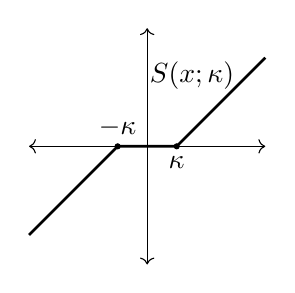
\begin{tikzpicture}[scale=1.5]
\draw[line width=1.0pt] (-1,-0.75)--(-0.25,0)--(0.25,0)--(1,0.75);
\draw [<->] (-1,0) -- (1,0);
\draw [<->] (-0,-1) -- (-0,1);
\filldraw (0.25,0) circle[radius={0.6*1.5/1.5pt}];
\filldraw (-0.25,0) circle[radius={0.6*1.5/1.5pt}];
\draw (-0.25,0) node[above] {$-\kappa$};
\draw (0.25,0) node[below] {$\kappa$};
\draw (0.38,0.6) node {$S(x;\kappa)$};
\end{tikzpicture}}
\end{center}
\end{frame}

\begin{frame}
\frametitle{Proximal operator example: Projection}
Projection onto nonempty closed convex $C\subseteq\reals^n$:
\[
\proj_C(y)=\argmin_{x\in C}\|x-y\|
\]
\vspace{0.2in}


Since $\prox_{\alpha \delta_C}
=\prox_{\delta_C}=\proj_C$
for any $\alpha>0$,
 proximal operators generalize projections.
\end{frame}

\begin{frame}
\frametitle{Proximable functions}
Evaluating $\prox_{\alpha f}$ is an optimization problem itself.
However, many interesting convex $f$ has a closed-form solution for $\prox_{\alpha f}$ so it is a useful subroutine.


\vspace{0.2in}
$f$ is proximable (informal definition) if $\prox_{\alpha f}$ is computationally efficient to evaluate.
Catalog of proximable functions in several papers.

\vspace{0.2in}

We decompose an optimization problem into smaller, simpler differentiable or proximable functions and operate on them separately.

\end{frame}



\end{document}
